\documentclass[10pt]{article}
\usepackage[polish]{babel}
\usepackage[utf8]{inputenc}
\usepackage[T1]{fontenc}
\usepackage{amsmath}
\usepackage{amsfonts}
\usepackage{amssymb}
\usepackage[version=4]{mhchem}
\usepackage{stmaryrd}
\usepackage{graphicx}
\usepackage[export]{adjustbox}
\graphicspath{ {./images/} }
\usepackage{hyperref}
\hypersetup{colorlinks=true, linkcolor=blue, filecolor=magenta, urlcolor=cyan,}
\urlstyle{same}

\title{GIMNAZJUM }

\author{}
\date{}


\newcommand\Varangle{\mathop{{<\!\!\!\!\!\text{\small)}}\:}\nolimits}

%New command to display footnote whose markers will always be hidden
\let\svthefootnote\thefootnote
\newcommand\blfootnotetext[1]{%
  \let\thefootnote\relax\footnote{#1}%
  \addtocounter{footnote}{-1}%
  \let\thefootnote\svthefootnote%
}

%Overriding the \footnotetext command to hide the marker if its value is `0`
\let\svfootnotetext\footnotetext
\renewcommand\footnotetext[2][?]{%
  \if\relax#1\relax%
    \ifnum\value{footnote}=0\blfootnotetext{#2}\else\svfootnotetext{#2}\fi%
  \else%
    \if?#1\ifnum\value{footnote}=0\blfootnotetext{#2}\else\svfootnotetext{#2}\fi%
    \else\svfootnotetext[#1]{#2}\fi%
  \fi
}

\begin{document}
\maketitle
\begin{enumerate}
  \item Liczby dodatnie \(a, b\) spełniają warunek
\end{enumerate}

\[
\frac{a+b}{2}=\sqrt{a b+3}
\]

Wykaż, że co najmniej jedna z liczb \(a, b\) jest niewymierna.\\
2. W każde pole tablicy o wymiarach \(4 \times 4\) wpisano liczbę 0 lub 1. Następnie obliczono sumy liczb stojących w każdym wierszu, w każdej kolumnie i na obu przekątnych. Wykaż, że co najmniej trzy sumy są jednakowe.\\
3. Punkt \(S\) leży wewnątrz sześciokąta foremnego \(A B C D E F\). Udowodnij, że suma pól trójkątów \(A B S, C D S, E F S\) jest równa połowie pola sześciokąta \(A B C D E F\).

\section*{LICEUM}
\begin{enumerate}
  \item Wykazać, że jeśli liczby całkowite \(a, b, c\) spełniają równanie
\end{enumerate}

\[
(a+3)^{2}+(b+4)^{2}-(c+5)^{2}=a^{2}+b^{2}-c^{2}
\]

to wspólna wartość obu stron jest kwadratem liczby całkowitej.\\
2. Na bokach \(B C\) i \(C A\) trójkąta \(A B C\) zbudowano po jego zewnętrznej stronie kwadraty \(B C D E\) oraz \(C A F G\). Prosta przechodząca przez punkt \(C\) i prostopadła do prostej \(D G\) przecina odcinek \(A B\) w punkcie \(M\). Udowodnić, że \(A M=M B\).\\
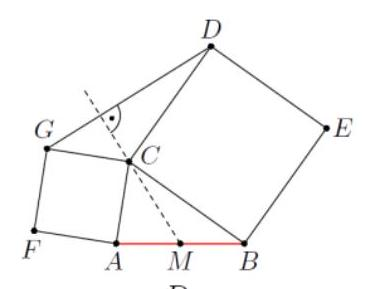
\includegraphics[max width=\textwidth, center]{2024_11_21_c750fbb4506b4f08fcb4g-1(1)}\\
3. Na przeciwprostokątnej \(B C\) trójkąta prostokątnego \(A B C\) zbudowano po zewnętrznej stronie kwadrat \(B C D E\). Niech \(O\) będzie środkiem tego kwadratu. Wykazać, że \(\Varangle B A O=\Varangle C A O\).\\
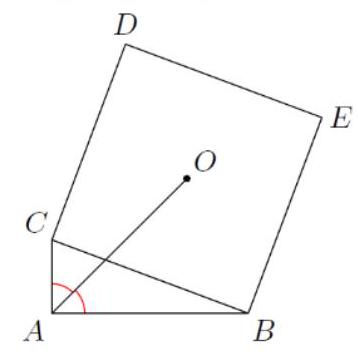
\includegraphics[max width=\textwidth, center]{2024_11_21_c750fbb4506b4f08fcb4g-1}

\footnotetext{Rozwiązania należy oddać do piątku 15 kwietnia do godziny 10.35 koordynatorowi konkursu panu Jarostawowi Szczepaniakowi lub swojemu nauczycielowi matematyki lub przestać na adres \href{mailto:jareksz@interia.pl}{jareksz@interia.pl} do piątku 15 kwietnia do pótnocy.
}
\end{document}